\selectlanguage{english}

As already noted in \secref{sssec:div}, the computation of Next-to-Leading Order (NLO) corrections often produces diverging amplitudes. However, this seems to be a consequence of Heisenberg's principle, implying that a quantum field theory cannot be valid at all energy scales at once.

\section{Renormalization of \texorpdfstring{$ \lambda \phi^4 $}{λφ4}-theory}

\subsection{1-Loop diagrams}
\label{ssec:f4-1-loop}

Consider $ \lambda \phi^4 $-theory and compute the scattering cross-section for $ \phi \phi \rightarrow \phi \phi $ at LO:
\begin{equation*}
  \begin{tikzpicture}[baseline=(r.base)]
    \begin{feynman}[inline=(r.base)]
      \vertex (a1) {};
      \vertex[right=4cm of a1] (a2) {};
      \vertex[below=4em of a1] (b1) {};
      \vertex[below=4em of a2] (b2) {};
      \vertex[below=2em of a1] (c1) {};
      \vertex[right=2cm of c1, dot] (c2) {};

      \vertex[below=2.2em of a1] (r);

      \diagram* {
        (a1) -- [scalar, momentum = \(p_1\)] (c2),
        (b1) -- [scalar, momentum' = \(p_2\)] (c2),
        (c2) -- [scalar, momentum = \(p_3\)] (a2),
        (c2) -- [scalar, momentum' = \(p_4\)] (b2),
      };
    \end{feynman}
  \end{tikzpicture}
  \qquad \Rightarrow \qquad
  \dd \sigma^\text{LO} = \frac{1}{\Phi} \frac{\dd^3p_3}{(2\pi)^3 2E_{p_3}} \frac{\dd^3p_4}{(2\pi)^4 2E_{p_4}} (2\pi)^4 \delta^{(4)}(p_1 + p_2 - p_3 - p_4) \lambda^2
\end{equation*}
In the CM frame:
\begin{equation*}
  p_1 = (E, 0, 0, p)
  \quad
  p_2 = (E, 0, 0, -p)
  \qquad
  p_3 = (E, p \sin \theta, 0, p \cos \theta)
  \quad
  p_4 = (E, -p \sin \theta, 0, - p \cos \theta)
\end{equation*}
\begin{equation*}
  s = 4E^2
  \qquad
  t = -2p^2 (1 + \cos \theta)
  \qquad
  u = -2p^2 (1 - \cos \theta)
\end{equation*}
with flux factor $ \Phi = 8pE $. Then the cross-section becomes:
\begin{equation*}
  \dd \sigma^\text{LO} = \frac{\lambda^2}{8pE} \frac{\dd^3p_3}{(2\pi)^2 (2E_{p_3})^2} \delta(2E - 2\sqrt{p_3^2 + m^2}) = \frac{\lambda^2}{8pE} \frac{p_3 \dd p_3 \dd \Omega_2}{(2\pi)^2 4E_{p_3}} \delta(E_{p_3} - E) = \frac{\lambda^2}{8pE} \frac{p}{16\pi E} \dd \cos \theta
\end{equation*}
Therefore, there's no angular dependence:
\begin{equation}
  \frac{\dd \sigma^\text{LO}}{\dd \cos \theta} = \frac{\lambda^2}{128 \pi} \frac{1}{E^2}
\end{equation}
Now, consider the NLO corrections to this cross-section, i.e. the 1-loop corrections:
\begin{equation*}
  \begin{tikzpicture}[baseline=(r.base)]
    \begin{feynman}[inline=(r.base)]
      \vertex (a1) {};
      \vertex[right=4cm of a1] (a2) {};
      \vertex[below=4em of a1] (b1) {};
      \vertex[below=4em of a2] (b2) {};
      \vertex[below=2em of a1] (c1) {};
      \vertex[right=2cm of c1, blob] (c2) {};

      \vertex[below=2.2em of a1] (r);

      \diagram* {
        (a1) -- [scalar, momentum = \(p_1\)] (c2),
        (b1) -- [scalar, momentum' = \(p_2\)] (c2),
        (c2) -- [scalar, momentum = \(p_3\)] (a2),
        (c2) -- [scalar, momentum' = \(p_4\)] (b2),
      };
    \end{feynman}
  \end{tikzpicture}
  \quad = \quad
  \begin{tikzpicture}[baseline=(r.base)]
    \begin{feynman}[inline=(r.base)]
      \vertex (a1) {};
      \vertex[right=4cm of a1] (a2) {};
      \vertex[below=4em of a1] (b1) {};
      \vertex[below=4em of a2] (b2) {};
      \vertex[below=2em of a1] (c1) {};
      \vertex[right=2cm of c1, dot] (c2) {};

      \vertex[below=2.2em of a1] (r);

      \diagram* {
        (a1) -- [scalar, momentum = \(p_1\)] (c2),
        (b1) -- [scalar, momentum' = \(p_2\)] (c2),
        (c2) -- [scalar, momentum = \(p_3\)] (a2),
        (c2) -- [scalar, momentum' = \(p_4\)] (b2),
      };
    \end{feynman}
  \end{tikzpicture}
  \quad + \smo(\lambda^2) \equiv -i \lambda F(s,t)
\end{equation*}
where $ F(s,t) $ is called \bctxt{form factor}.

\begin{proposition}{Form factor}{}
  In $ \lambda \phi^4 $-theory, the form factor at NLO is:
  \begin{equation}
    F(s,t) = 1 - i\lambda \left( V(s) + V(t) + V(u) \right) + \smo(\lambda^2)
  \end{equation}
  with:
  \begin{equation}
    V(p^2) \defeq \frac{1}{2} \int \frac{\dd^4k}{(2\pi)^4} \frac{i}{k^2 - m^2} \frac{i}{(p + k)^2 - m^2}
    \label{eq:vps-def}
  \end{equation}
\end{proposition}

\begin{proofbox}
  \begin{proof}
    The NLO correction to the scattering amplitude is given by three loop diagrams:
    \begin{equation*}
      \begin{tikzpicture}[baseline = (r.base)]
        \begin{feynman}[inline = (r.base)]
          \vertex (x1) {};
          \vertex[below=3em of x1] (p1) {};
          \vertex[below=3em of p1] (x2) {};

          \vertex[right=3em of p1, dot] (v1) {};
          \vertex[right=5em of v1, dot] (v2) {};

          \vertex[right=3em of v2] (p2) {};
          \vertex[above=3em of p2] (x3) {};
          \vertex[below=3em of p2] (x4) {};

          \vertex[above=0.5em of v1] (r) {};

          \diagram* {
            (x1) -- [scalar, momentum = \(p_1\)] (v1),
            (x2) -- [scalar, momentum' = \(p_2\)] (v1),
            (v2) -- [scalar, momentum = \(p_3\)] (x3),
            (v2) -- [scalar, momentum' = \(p_4\)] (x4),

            (v1) -- [scalar, half left, momentum' = \(p'\)] (v2),
            (v2) -- [scalar, half left, momentum' = \(p\)] (v1),
          };
        \end{feynman}
      \end{tikzpicture}
      \qquad
      \begin{tikzpicture}[baseline = (r.base)]
        \begin{feynman}[inline = (r.base)]
          \vertex (x1) {};
          \vertex[right=4em of x1] (p1) {};
          \vertex[right=4em of p1] (x3) {};

          \vertex[below=2em of p1, dot] (v1) {};
          \vertex[below=5em of v1, dot] (v2) {};

          \vertex[below=9em of x1] (x2) {};
          \vertex[below=9em of x3] (x4) {};

          \vertex[below=2em of v1] (r) {};

          \diagram* {
            (x1) -- [scalar, momentum = \(p_1\)] (v1) -- [scalar, momentum = \(p_3\)] (x3),
            (x2) -- [scalar, momentum' = \(p_2\)] (v2) -- [scalar, momentum' = \(p_4\)] (x4),

            (v1) -- [scalar, half left, momentum = \(p + p_1 - p_3\)] (v2),
            (v2) -- [scalar, half left, momentum = \(p\)] (v1),
          };
        \end{feynman}
      \end{tikzpicture}
      \qquad
      \begin{tikzpicture}[baseline = (r.base)]
        \begin{feynman}[inline = (r.base)]
          \vertex (x1) {};
          \vertex[right=4em of x1] (p1) {};
          \vertex[right=4em of p1] (x3) {};

          \vertex[below=2em of p1, dot] (v1) {};
          \vertex[below=5em of v1, dot] (v2) {};

         \vertex[below=9em of x1] (x2) {};
          \vertex[below=9em of x3] (x4) {};

          \vertex[below=2em of v1] (r) {};

          \diagram* {
            (x1) -- [scalar, momentum = \(p_1\)] (v1) -- [scalar, momentum = \(p_4\)] (x3),
            (x2) -- [scalar, momentum' = \(p_2\)] (v2) -- [scalar, momentum' = \(p_3\)] (x4),

            (v1) -- [scalar, half left, momentum = \(p + p_1 - p_4\)] (v2),
            (v2) -- [scalar, half left, momentum = \(p\)] (v1),
          };
        \end{feynman}
      \end{tikzpicture}
    \end{equation*}
    with $ p' = p_1 + p_2 + p $. These correspond to loop diagrams in the $ s $, $ t $ and $ u $ channels, therefore, recalling \eref{eq:f4-loop-ampl}, the thesis is trivially found.
  \end{proof}
\end{proofbox}

\begin{lemma}[before upper = {\tcbtitle}]{Feynman parameters}{}
  \begin{equation}
    \frac{1}{AB} = \int_0^1 \dd x \frac{1}{\left( x A + (1-x) B \right)^2}  
  \end{equation}
\end{lemma}

This allows to rewrite $ V(p^2) $:
\begin{equation*}
  V(p^2) = - \frac{1}{2} \int \frac{\dd^4k}{(2\pi)^4} \int_0^1 \dd x \left[ k^2 - m^2 + x \left( 2 k \cdot p + p^2 \right) \right]^{-2} \equiv - \frac{1}{2} \int_0^1 \dd x \int \frac{\dd^4\ell}{(2\pi)^4} \frac{1}{\left( \ell^2 - M^2 \right)^2}
\end{equation*}
having defined:
\begin{equation}
  \ell \equiv k + x p
  \qquad \qquad
  M^2 \equiv m^2 - x (1-x) p^2
\end{equation}

\begin{lemma}[before upper = {\tcbtitle}]{}{}
  \begin{equation}
    I_d(n) \equiv \int \frac{\dd^dk}{(2\pi)^d} \frac{1}{(k^2 - M^2 + i\epsilon)^n} = \frac{i (-1)^n}{(4\pi)^{d/2}} \frac{\Gamma(n - \frac{d}{2})}{\Gamma(n)} \left( \frac{1}{M^2} \right)^{n - d/2}
    \label{eq:int-dn}
  \end{equation}
\end{lemma}

\begin{proofbox}
  \begin{proof}
    The poles of the integrand function are $ k_0 = \pm \left[ \sqrt{M^2 + \ve{k}^2} - i\epsilon \right] $, therefore the integration path $ I = \R $ can be rotated counterclockwise by $ \frac{\pi}{2} $ without overlapping with any pole. The resulting Wick rotation $ k_0 \mapsto i k_0 $, i.e. $ k \mapsto k_\text{E} $ implies $ k_E \in \R $, therefore the $ d $-dimensional integral in Minkowskian metric becomes a $ d $-dimensional integral with (negative) Euclidean metric:
    \begin{equation*}
      I_d(n) = i (-1)^n \int \frac{\dd^dk_\text{E}}{(2\pi)^d} \frac{1}{(k_\text{E}^2 + M^2 - i\epsilon)^n} = i (-1)^n \int_{\mathbb{S}^d} \dd \Omega_d \int_{\R^+} \dd k_\text{E} \frac{k_\text{E}^{d-1}}{(k_\text{E}^2 + M^2)^n}
    \end{equation*}
    It can be shown that:
    \begin{equation}
      \int_{\R^+} \dd k_\text{E} \frac{k_\text{E}^{d-1}}{(k_\text{E}^2 + M^2)^n} = \frac{1}{2} \frac{\Gamma(n - \frac{d}{2}) \Gamma(\frac{d}{2})}{\Gamma(n)} \left( \frac{1}{M^2} \right)^{n - \frac{d}{2}}
    \end{equation}
    Inserting \eref{eq:solid-angle} yields the thesis.
  \end{proof}
\end{proofbox}

\eref{eq:int-dn} diverges for $ (d,n) = (4,2) $, as $ \Gamma(z) = \frac{1}{z} - \gamma_\text{E} + o(z) $, therefore a cutoff needs to be introduced to regularize the integral:
\begin{equation*}
  \begin{split}
    V(p^2)
    & = \lim_{\Lambda \rightarrow \infty} \frac{-i}{2} \int_0^1 \dd x \int_0^\Lambda \frac{\dd k_\text{E}}{8\pi^2} \frac{k_\text{E}^3}{(k_\text{E}^2 + M^2)^2} = \lim_{\Lambda \rightarrow \infty} \frac{-i}{2} \int_0^1 \dd x \int_{M^2}^{\Lambda^2 + M^2} \frac{\dd \rho}{16\pi^2} \frac{\rho - M^2}{\rho^2} \\
    & = \lim_{\Lambda \rightarrow \infty} \frac{-i}{32 \pi^2} \int_0^1 \dd x \left[ \log \left( 1 + \frac{\Lambda^2}{M^2} \right) - \frac{\Lambda^2}{\Lambda^2 + M^2} \right] \\
    & = \lim_{\Lambda \rightarrow \infty} \frac{-i}{32\pi^2} \int_0^1 \dd x \left[ \log \frac{\Lambda^2}{M^2} - 1 + \smo  \left( \frac{M^2}{\Lambda^2} \right) \right]
  \end{split}
\end{equation*}
The form factor can then be rewritten as:
\begin{equation}
  F(s,t) = 1 + \frac{\lambda}{32\pi^2} \left[ 3 + \lim_{\Lambda \rightarrow \infty} \int_0^1 \dd x \left( \log \frac{M^2(s)}{\Lambda^2} + \log \frac{M^2(t)}{\Lambda^2} + \log \frac{M^2(u)}{\Lambda^2} \right) \right] + \smo(\lambda^2)
  \label{eq:form-factor}
\end{equation}
Now, define the threshold values $ s_0 \equiv 4m^2 $, $ t_0 = u_0 \equiv 0 $. The \bctxt{physical coupling constant} $ \lambda_\text{phys} $ is defined as:
\begin{equation}
  \frac{\dd \sigma}{\dd \cos \theta}\bigg\vert_{s_0 , t_0} = \frac{\lambda_\text{phys}^2}{128\pi m^2}
\end{equation}
which is linked to the \bctxt{bare coupling constant} $ \lambda_\text{bare} \equiv \lambda $ by:
\begin{equation}
  \lambda_\text{bare} F(s_0,t_0) = \lambda_\text{phys}
  \label{eq:bare-phys-def}
\end{equation}

\begin{proposition}{Bare and physical coupling}{bare-phys-coupl}
  The NLO form factor can be expressed as:
  \begin{equation}
    \lambda F(s,t) = \lambda_\text{phys} \left[ 1 - \frac{\lambda_\text{phys}}{32\pi^2} \int_0^1 \dd x \left( \log \frac{M^2(s)}{M^2(s_0)} + \log \frac{M^2(t)}{M^2(t_0)} + \log \frac{M^2(u)}{M^2(u_0)} \right) \right] + \smo(\lambda_\text{phys}^3)
    \label{eq:l-f-cutoff}
  \end{equation}
\end{proposition}

\begin{proofbox}
  \begin{proof}
    By \eref{eq:bare-phys-def}:
    \begin{equation*}
      \lambda_\text{phys} = \lambda (1 - c_0 \lambda) + \smo(\lambda^3)
      \qquad \Leftrightarrow \qquad
      \lambda = \lambda_\text{phys} (1 + c_0 \lambda_\text{phys}) + \smo(\lambda_\text{phys}^3)
    \end{equation*}
    Therefore:
    \begin{equation*}
      \lambda (1 - c \lambda) = \lambda_\text{phys} (1 + c_0 \lambda_\text{phys}) (1 - c \lambda_\text{phys}) + \smo(\lambda_\text{phys}^3) = \lambda_\text{phys} (1 - (c - c_0) \lambda_\text{phys}) + \smo(\lambda_\text{phys}^3)
    \end{equation*}
    Inserting \eref{eq:form-factor} yields the thesis.
  \end{proof}
\end{proofbox}

Expressing $ \lambda_\text{bare} $ as a function of $ \lambda_\text{phys} $ eliminates the divergence regularized by the cutoff, which is absorbed into $ \lambda_\text{phys} $, which is the observable coupling constant. Note that the choice of $ s_0 $ and $ t_0 $ to define $ \lambda_\text{phys} $ is purely conventional: a more useful choice is imposing:
\begin{equation}
  M^2(s_0) = M^2(t_0) = M^2(u_0) = \mu^2
\end{equation}
It is important to stress the difference between $ \Lambda $ and $ \mu $: $ \Lambda $ is a \bctxt{regularization scale}, introduced to regularize diverging loop integrals, while $ \mu $ is a \bctxt{renormalization point}, introduced to eliminate the $ \Lambda $-depedence\footnotemark. Both parameters are arbitrary, hence physical observables cannot depend on any of them: this means that the explicit $ \mu $-dependence of $ F(s,t) $ must cancel the implicit $ \mu $-dependence of $ \lambda $, so that $ \lambda_\text{phys} $. \\
The infinities which cancel expressing $ F(s,t) $ in terms of $ \lambda_\text{phys} $ are explicit when expressing $ \lambda_\text{bare} = \lambda_\text{bare}(\lambda_\text{phys}) $. In fact:
\begin{equation*}
  \lambda_\text{phys} = \lambda_\text{bare} \left[ 1 + \frac{3\lambda_\text{bare}}{32\pi^2} \left( 1 + \log \frac{\mu^2}{\Lambda^2} \right) \right] + \smo(\lambda_\text{bare}^3)
\end{equation*}
Thus, choosing $ \mu^2 \propto \Lambda^2 $, it is possible to express $ \lambda_\text{phys} $ as a limit of $ \lambda_\text{bare} $, and eventually $ \lambda_\text{phys} = \lambda_\text{bare} $: the bare coupling constant is the physical coupling at the scale $ \Lambda \rightarrow \infty $ (infinitely-small distances), i.e. including the fluctuations at all scales. Due to Heisenberg's principle, then, $ \lambda_\text{bare} $ is expected to diverge: excitations of the fields in momentum space are defined as normal coordinates of the system in position space, i.e. $ p \sim \pa_x \phi \sim \frac{1}{\Delta x} $, which diverges as $ \Delta x \rightarrow 0 $ (as $ \Lambda \rightarrow \infty $).

\footnotetext{The regularization scale $ \Lambda $ is an unphysical artifact introduce to isolate UV divergences, it depends on the specific regularization scheme adopted (UV cut-off, dimensional regolarization, etc.) and it disappears in renormalized results, while the renormalization point $ \mu $ is the physical reference scale which defines renormalized physical parameters.}

\subsection{Renormalized perturbation theory}

The process of renormalization, which allows to obtain finite results from diverging amplitudes, can be implemented in various ways. That of introducing a UV cut-off $ \Lambda $, expressing the bare observables in terms of the physical observables at some scale $ \mu $ and then setting $ \Lambda \rightarrow \infty $ is rather inefficient at higher orders in perturbation theory: thus, a more efficient renormalization scheme must be adopted. \\
First of all, substitute the UV cut-off with a \bctxt{dimensional regularization scheme} ('t Hooft--Veltman scheme): this scheme consists in turning diverging loop integrals into meromorphic\footnotemark functions of $ d \in \C $, which is an analytic continuation of the number of spacetime dimensions. In particular:
\begin{equation}
  d = 4 - 2 \epsilon
\end{equation}
with $ \epsilon \in \C : \Re{\epsilon} < 0 $. By analytic continuation of the Lagrangian of the theory, the dimensionality of the various objects changes.

\footnotetext{Given an open set $ D \subset \C $, then $ f : D \rightarrow \C $ is \textit{meromorphic} if it is holomorphic on $ D - P $, where $ P \subset D $ is a set of isolated points called \textit{poles}. Recall that a function $ f : D \rightarrow \C $ is \textit{holomorphic} on $ D $ if it is complex differentiable at every point in $ D $.}

\begin{proposition}{Dimensional analysis}{}
  In $ d = 4 $:
  \begin{equation}
    [\phi] = [M]
    \qquad \qquad
    [\lambda] = 1
  \end{equation}
\end{proposition}

\begin{proofbox}
  \begin{proof}
    In natural units $ \hbar = c = 1 $, each physical quantity has the dimension of a power of mass, as:
    \begin{equation*}
      [\hbar] = [E] [T] = [M] [T] \equiv 1
      \qquad \qquad
      [c] = [L] [T]^{-1} \equiv 1
    \end{equation*}
    where $ E = m $ ($ c^2 = 1 $) was used. Therefore, $ [L] = [T] = [M]^{-1} $. In this system, the action must be a dimensionless quantity:
    \begin{equation*}
      \act = \int \dd^4x \,\lag
      \qquad \Rightarrow \qquad
      1 = [L]^4 [\lag] = [M]^{-4} [\lag]
      \qquad \Rightarrow \qquad
      [\lag] = [M]^4
    \end{equation*}
    As $ [\pa_\mu] = [L]^{-1} = [M] $, then, it is clear that $ [\phi] = [M] $ and, being $ \lag_\text{int} = - \frac{\lambda}{4!} \phi^4 $, $ [\lambda] = 1 $.
  \end{proof}
\end{proofbox}

\begin{proposition}{Dimensionality in 't Hooft--Veltman scheme}{}
  In $ d = 4 - 2\epsilon $:
  \begin{equation}
    [\phi] = [M]^{1 - \epsilon}
    \qquad \qquad
    [\lambda] = [M]^{2\epsilon}
  \end{equation}
\end{proposition}

\begin{proofbox}
  \begin{proof}
    In the dimensional regularization scheme the differential becomes $ \dd^4x \mapsto \dd^dx $, therefore the Lagrangian must have:
    \begin{equation*}
      [\lag] = [M]^d = [M]^{4 - 2\epsilon}
    \end{equation*}
    $ [\pa_\mu] = [M] $ remains unchanged, therefore $ [\phi] = [M]^{1 - \epsilon} $ and, as a consequence, $ [\lambda] = [M]^{2\epsilon} $.
  \end{proof}
\end{proofbox}

To explicit the dimensionality of the (bare) coupling constant, a regularization scale $ \mu_\text{reg} $ is introduced, so that:
\begin{equation}
  \lambda = \mu_\text{reg}^{2\epsilon} \lambda_\text{bare}
\end{equation}

\begin{proposition}{}{}
  In $ d = 4 - 2\epsilon $:
  \begin{equation}
    -i \lambda V(p^2) = - \frac{\lambda_\text{bare}}{32\pi^2} \int_0^1 \dd x \left[ \frac{1}{\epsilon} - \gamma_\text{E} + \ln 4\pi - \log \frac{M^2}{\mu_\text{reg}^2} + \smo(\epsilon) \right]
  \end{equation}
  where $ \gamma_\text{E} \simeq 0.5772 $ is the Euler--Mascheroni constant.
\end{proposition}

\begin{proofbox}
  \begin{proof}
    From \eref{eq:vps-def} and using \eref{eq:int-dn}:
    \begin{equation*}
      \begin{split}
        -i \lambda V(p^2)
        & = \frac{i \lambda}{2} \int_0^1 \dd x \int \frac{\dd^d\ell}{(2\pi)^d} \frac{1}{(\ell^2 - M^2)^2} = \frac{i \lambda_\text{bare}}{2} \mu_\text{reg}^{2\epsilon} \int_0^1 \dd x \frac{i}{(4\pi)^{2 - \epsilon}} \frac{\Gamma(\epsilon)}{2} (M^2)^{-\epsilon} \\
        & = - \frac{\lambda_\text{bare}}{32\pi^2} \int_0^1 \dd x \, (4\pi)^\epsilon \Gamma(\epsilon) \left( \frac{M^2}{\mu_\text{reg}^2} \right)^{-\epsilon}
      \end{split}
    \end{equation*}
    Now, the Laurent series in $ \epsilon $ for this expression is:
    \begin{equation*}
      \begin{split}
        -i \lambda V(p^2)
        &= - \frac{\lambda_\text{bare}}{32\pi^2} \int_0^1 \dd x \left( 1 + \epsilon \log 4\pi + \smo(\epsilon) \right) \left( \frac{1}{\epsilon} - \gamma_\text{E} + \smo(\epsilon) \right) \left( 1 - \epsilon \log \frac{M^2}{\mu_\text{reg}^2} + \smo(\epsilon) \right) \\
        & = - \frac{\lambda_\text{bare}}{32\pi^2} \int_0^1 \dd x \left[ \frac{1}{\epsilon} - \gamma_\text{E} + \log 4\pi - \log \frac{M^2}{\mu_\text{reg}^2} + \smo(\epsilon) \right]
      \end{split}
    \end{equation*}
    which is the thesis.
  \end{proof}
\end{proofbox}

The dimensionally-regularized form factor, then, takes the form:
\begin{equation*}
  F(s,t) = 1 - \frac{\lambda_\text{bare}}{32\pi^2} \left[ 3 \left( \frac{1}{\epsilon} - \gamma_\text{E} + \log 4\pi \right) - \int_0^1 \dd x \left( \log \frac{M^2(s)}{\mu_\text{reg}^2} + \log \frac{M^2(t)}{\mu_\text{reg}^2} + \log \frac{M^2(u)}{\mu_\text{reg}^2} \right) \right] + \smo(\epsilon)
\end{equation*}
It would then be possible to proceed with the renormalization of the coupling constant specifying a cinematic $ (s_0,t_0) $ and setting $ \lambda_\text{phys} = \lambda_\text{bare} F(s_0,t_0) $. However, given the arbitrariness of the renormalization point $ \mu_\text{ren} $, it is algebrically convenient to choose an unphysical cinematic which simplifies the expression of $ \lambda_\text{phys} $.

\begin{definition}{Minimal subtraction scheme}{}
  The \bcdef{minimal subtraction scheme} (MS) is a renormalization scheme with renormalization point such that:
  \begin{equation}
    \lambda_\text{MS} = \lambda_\text{bare} \left[ 1 - \frac{3\lambda_\text{bare}}{32\pi^2} \frac{1}{\epsilon} \right] + \smo(\lambda_\text{bare}^3)
  \end{equation}
\end{definition}

When working with dimensional regularization, it is more useful to adopt the \bctxt{modified MS scheme} ($ \msb $), which includes the universal constant $ -\gamma_\text{E} + \log 4\pi $ in the expression for the physical coupling constant:
\begin{equation}
  \lambda_{\msb} = \lambda_\text{bare} \left[ 1 - \frac{3\lambda_\text{bare}}{32\pi^2} \left( \frac{1}{\epsilon} - \gamma_\text{E} + \log 4\pi \right) \right] + \smo(\lambda_\text{bare}^3)
  \label{eq:l-msb}
\end{equation}

\begin{theorem}{Scales in the $ \msb $ scheme}{}
  In the $ \msb $ scheme:
  \begin{equation}
    \mu_\text{reg} = \mu_\text{ren}
  \end{equation}
\end{theorem}

\begin{proofbox}
  \begin{proof}
    As of \eref{eq:l-msb}, using the same reasoning as in the proof of \pref{prop:bare-phys-coupl}:
    \begin{equation}
      \lambda_\text{bare} = \lambda_{\msb} \left[ 1 + \frac{3\lambda_{\msb}}{32\pi^2} \left( \frac{1}{\epsilon} - \gamma_\text{E} + \log 4\pi \right) \right] + \smo(\lambda_{\msb}^3)
    \end{equation}
    Moreover:
    \begin{equation*}
      \begin{split}
        \lambda_\text{bare} F(s,t)
        & = \lambda_\text{bare} \left[ 1 - \frac{3\lambda_\text{bare}}{32\pi^2} \left( \frac{1}{\epsilon} - \gamma_\text{E} + \log 4\pi \right) \right] \\
        & \qquad \qquad \qquad \qquad  + \frac{\lambda_\text{bare}^2}{32\pi^2} \int_0^1 \dd x \left( \log \frac{M^2(s)}{\mu_\text{reg}^2} + \log \frac{M^2(t)}{\mu_\text{reg}^2} + \log \frac{M^2(u)}{\mu_\text{reg}^2} \right) + \smo(\lambda_\text{bare}^3) \\
      \end{split}
    \end{equation*}
    Then, noting that $ \lambda_\text{bare}^2 = \lambda_{\msb}^2 + \smo(\lambda_{\msb}^3) $:
    \begin{equation*}
      \lambda_\text{bare} F(s,t) = \lambda_{\msb} \left[ 1 + \frac{\lambda_{\msb}}{32\pi^2} \int_0^1 \dd x \left( \log \frac{M^2(s)}{\mu_\text{reg}^2} + \log \frac{M^2(t)}{\mu_\text{reg}^2} + \log \frac{M^2(u)}{\mu_\text{reg}^2} \right) \right] + \smo(\lambda_{\msb}^3)
    \end{equation*}
    Comparing this expression to \eref{eq:l-f-cutoff}, it is clear that $ \mu_\text{reg} $ is also the renormalization point of the scheme.
  \end{proof}
\end{proofbox}

Hence, in the $ \msb $ scheme $ \mu_\text{reg} = \mu_\text{ren} \equiv \mu $.

\subsubsection{Lagrangian counterterms}
\label{sssec:lag-count}

Define $ Z_\lambda : \lambda_\text{bare} = Z_\lambda \lambda_{\msb} \equiv \lambda_{\msb} + \delta_\lambda $, so that:
\begin{equation*}
  Z_\lambda = 1 + \frac{3\lambda_{\msb}}{32\pi^2} \left( \frac{1}{\epsilon} - \gamma_\text{E} + \log 4\pi \right) + \smo(\lambda_{\msb}^2)
  \qquad
  \delta_\lambda = 1 + \frac{3\lambda_{\msb}}{32\pi^2} \left( \frac{1}{\epsilon} - \gamma_\text{E} + \log 4\pi \right) + \smo(\lambda_{\msb}^3)
\end{equation*}
Inserting into the Lagrangian:
\begin{equation*}
  \begin{split}
    \lag
    & = \frac{1}{2} \left( \pa_\mu \phi \pa^\mu \phi - m^2 \phi^2 \right) - \frac{\lambda}{4!} \phi^4 \\
    & = \frac{1}{2} \left( \pa_\mu \phi \pa^\mu \phi - m^2 \phi^2 \right) - \frac{\lambda_{\msb}}{4!} \phi^4 - \frac{\delta_\lambda}{4!} \phi^4 + \smo(\lambda_{\msb}^3)
  \end{split}
\end{equation*}
It is then clear that renormalizing the coupling constant is equivalent to adding a counterterm to the Lagrangian, which contains the original divergence. This counterterm induces a new interaction vertex:
\begin{equation}
  \begin{tikzpicture}[baseline=(r.base)]
    \begin{feynman}[inline=(r.base)]
      \vertex (a1) {};
      \vertex[right=4cm of a1] (a2) {};
      \vertex[below=4em of a1] (b1) {};
      \vertex[below=4em of a2] (b2) {};
      \vertex[below=2em of a1] (c1) {};
      \vertex[right=2cm of c1, crossed dot] (c2) {};

      \vertex[below=2.2em of a1] (r);

      \diagram* {
        (a1) -- [scalar] (c2),
        (b1) -- [scalar] (c2),
        (c2) -- [scalar] (a2),
        (c2) -- [scalar] (b2),
      };
    \end{feynman}
  \end{tikzpicture}
  \quad = \quad -i \delta_\lambda
  \label{eq:counterterm}
\end{equation}
This process is general: divergences are cured order by order in perturbation theory by adding each time new counterterms to the Lagrangian: hence the name of renormalized perturbation theory\footnote{The name may be confusing, as the counterterms still contain divergences.}. At each order, each new counterterms are fixed by an appropriate physical condition.

\subsection{Renormalizability}

The problem of renormalization has been reduced to that of classifying all possible counterterms to the Lagrangian, where each counterterm arises from the normalization of a different class of diverging Feynman diagrams.

\begin{definition}{Superficial degree of divergence}{}
  Given a scalar field theory in $ d $ dimensions, the \bcdef{superficial degree of divergence} of a Feynman diagram with $ L $ loops and $ P_\text{s} $ scalar propagators is:
  \begin{equation}
    D \defeq d L - 2 P_\text{s}
    \label{eq:sup-deg-div-def}
  \end{equation}
\end{definition}

The superficial degree of divergence gives an idea of how badly the considered diagram diverges: indeed, each loop corresponds to an integration with measure $ \dd^dk $, which has dimension $ [M]^d $, and each propagator corresponds to a factor of $ \tilde{D}_\text{F}(p) \sim (p^2 - m^2)^{-1} $, which has dimension $ [M]^{-2} $, so $ D $ is the net power of momentum present in the amplitude:
\begin{equation*}
  \mat \sim \int \frac{\dd k}{k^{1-D}}
\end{equation*}
Introducing a UV cut-off $ \Lambda $, the divergence will be different for different values of $ D $:
\begin{itemize}
  \item $ D > 0 $: $ \mat \sim \Lambda^D $, hence the diagram has a UV divergence which must be renormalized;
  \item $ D = 0 $: $ \mat \sim \log \Lambda $, hence the diagram has a logarithmic UV divergence;
  \item $ D < 0 $: $ \mat \sim \Lambda^{-\abs{D}} $, hence the diagram is UV finite.
\end{itemize}
This, however, is a naive analysis: in fact, the diagram may have diverging sub-diagrams which make the actual degree of divergence worse, or it may have symmetries which make divergences partially cancel, leaving a better degree of divergence. As an example, a trivial diagram with no loops and no propagators has $ D = 0 $, but it is not a diverging diagram. \\
The problem of diverging sub-diagrams requires a more careful analysis. Consider the following diagram in $ 4 $-dimensional $ \lambda \phi^4 $-theory:
\begin{equation*}
  \begin{tikzpicture}[baseline = (r.base)]
    \begin{feynman}[inline = (r.base)]
      \vertex (a1) {};
      \vertex[right=1.3cm of a1] (a2) {};
      \vertex[right=1.3cm of a2] (a3) {};

      \vertex[above=1.3cm of a2, dot] (b1) {};
      \vertex[above=2.6cm of b1, dot] (b2) {};

      \vertex[above=1.3cm of b2] (c2) {};
      \vertex[left=1.3cm of c2, dot] (c1) {};
      \vertex[above=1.3cm of c1] (c4) {};
      \vertex[right=1.3cm of c2, dot] (c3) {};
      \vertex[above=1.3cm of c3] (c5) {};

      \vertex[left=1.3cm of c1] (d1) {};
      \vertex[above=1.3cm of d1] (d2) {};
      \vertex[right=1.3cm of c3] (d3) {};
      \vertex[above=1.3cm of d3] (d4) {};

      \vertex[below=0.5cm of b2] (r) {};

      \diagram* {
        (a1) -- [scalar] (b1) -- [scalar] (a3),
        (b1) -- [scalar, half left] (b2) -- [scalar, half left] (b1),
        (b2) -- [scalar] (c1) -- [scalar] (d2),
        (b2) -- [scalar] (c3) -- [scalar] (d4),
        (c4) -- [scalar] (c1) -- [scalar] (c3) -- [scalar] (c5),
      };
    \end{feynman}
  \end{tikzpicture}
  \qquad \qquad
  D = 4 \cdot 2 - 2 \cdot 5 = -2
\end{equation*}
Although $ D < 0 $, the loop integral diverges: however, in renormalized perturbation theory this divergence is cured by the counterterm \eref{eq:counterterm} This is a general property: apart from superficially divergent diagrams, the only other divergences arise from diverging sub-diagrams of superficially finite diagrams, but these divergences are cured by the counterterms already added to the Lagrangian. Hence, the renormalization procedure correctly cures all UV divergences.

\begin{theorem}{Bogolyubov--Parasyuk theorem}{}
  For any renormalized quantum field theory, the perturbative expansion of matrix elements of the $ S $-matrix is UV-finite.
\end{theorem}

\begin{proofbox}
  \begin{proof}
    The proof is found in \cite{bog-par, azp}.
  \end{proof}
\end{proofbox}

\subsubsection{\texorpdfstring{$ \lambda \phi^n $}{λφn}-theory}

\begin{lemma}{Loop number}{}
  Given a diagram with $ P $ propagators and $ V $ vertices, then:
  \begin{equation}
    L = P - V + 1
    \label{eq:loop-num}
  \end{equation}
\end{lemma}

\begin{proofbox}
  \begin{proof}
    Each loop is associated to an unconstrained momentum: each propagator corresponds to a momentum, while each vertex to a $ \delta $ which constrains the momenta of the diagram, but there's also an overall momentum-conserving $ \delta $ which makes one of the vertex-associated $ \delta $ redundant, hence $ L = P - (V - 1) $, which is the thesis.
  \end{proof}
\end{proofbox}

This result is valid in general for any field theory, and $ P $ represents the total number of propagators (even of different kinds). \\
Considering the specific case of $ \lambda \phi^n $-theory, instead, there's another relation which can simplify the computation of the superficial degrees of freedom: as each vertex has $ n $ scalar lines, then:
\begin{equation}
  n V = 2 P_\text{s} + N_\text{s}
  \label{eq:fn-v}
\end{equation}
where $ N_\text{s} $ is the number of external scalar lines. This expression takes into account the fact that each propagator links two vertices.

\begin{theorem}{Superficial degree of divergence}{lfn-sup-deg-div}
  In $ \lambda \phi^n $-theory in $ d $ dimensions, the \bcth{superficial degree of divergence} is:
    \begin{equation}
      D = d + \left( n \frac{d - 2}{2} - d \right) V - \frac{d - 2}{2} N
      \label{eq:lfn-sup-deg-div}
    \end{equation}
\end{theorem}

\begin{proofbox}
  \begin{proof}
    By \eref{eq:fn-v} $ P = \frac{1}{2} (n V - N) $, thus by \eref{eq:loop-num}:
    \begin{equation*}
      L = \left( \frac{n}{2} - 1 \right) V - \frac{N}{2} + 1
    \end{equation*}
    Recalling \eref{eq:sup-deg-div-def}:
    \begin{equation*}
      D = d \left[ \left( \frac{n}{2} - 1 \right) V - \frac{N}{2} + 1 \right] - n V + N = d + \left( n \frac{d - 2}{2} - d \right) V - \frac{d - 2}{2} N
    \end{equation*}
    which is the thesis.
  \end{proof}
\end{proofbox}

\begin{example}{$ \lambda \phi^4 $-theory}{p4-th}
  The case of $ \lambda \phi^4 $-theory in $ 4 $ dimensions is a particularly simple one, as:
  \begin{equation}
    D = 4 - N
  \end{equation}
  Hence, the only classes of diverging diagrams are vacuum-to-vacuum diagrams, which diverge as $ \sim \Lambda^4 $, the $ 1 \rightarrow 1 $ diagrams (i.e. the $ 2 $-point Green function of the theory and all its possible loop corrections), which diverges as $ \sim \Lambda^2 $, and the $ 2 \rightarrow 2 $ scattering, which diverges as $ \sim \log \Lambda $ (agreeing with \eref{eq:form-factor}). In this case there is only a finite number of classes of diverging diagrams.
\end{example}

\tref{th:lfn-sup-deg-div} can be derived also with dimensional analysis alone. In $ d $-dimensional $ \lambda \phi^n $-theory, it is trivial to show that:
\begin{equation*}
  [\phi] = [M]^{\frac{d - 2}{2}}
  \qquad \qquad
  [\lambda] = [M]^{d - n \frac{d - 2}{2}}
\end{equation*}
The dimensionality of $ \lambda $ is the dimensionality of a diagram with a single vertex, i.e. with $ N = n $ amputated legs, and, as diagrams with the same $ N $ have the same dimensionality, of any diagram with $ N = n $: generalizing, the dimensionality of a diagram with $ N $ amputated legs should be $ d - N \frac{d - 2}{2} $. On the other hand, if the diagram has $ V $ vertices, by definition it should have dimension $ [d]^V [M]^D $, thus:
\begin{equation*}
  \left( d - n \frac{d - 2}{2} \right) V + D = d - N \frac{d - 2}{2}
\end{equation*}
which is exactly \eref{eq:lfn-sup-deg-div}. It is then clear that $ D $ decreases as $ V $ increases (i.e. going to higher orders in perturbation theory) if and only if the coupling constant has positive mass dimension, leaving with only three possible classes theories:
\begin{itemize}
  \item super-renormalizable theories: the coupling constant has strictly negative mass dimension, hence there is only a finite number of diverging diagrams.
  \item renormalizable theories: the coupling constant is dimensionless, hence there is only a finite number of classes of diverging diagrams (although their absolute number may be infinite);
  \item non-renormalizable theories: the coupling constant has strictly negative mass dimension, hence there is an infinite number of diverging classes of diagrams.
\end{itemize}
Note that this are general properties, not restricted to real scalar field theories.

\begin{example}{$ d = 4 $ theories}{}
  Consider $ \lambda \phi^n $-theory in $ d = 4 $ dimensions. The coupling constant in $ \lag_\text{int} = - \frac{1}{n!} \lambda \phi^n $ has dimension $ 4 - n $, hence:
  \begin{itemize}
    \item $ \lambda \phi^3 $-theory is super-renormalizable: $ D = 4 - V - N $, thus the only diverging diagrams are the $ 2 $-point Green function (loop corrections have $ D < 0 $) and the single interaction vertex, while all other diagrams have a finite amplitude;
    \item $ \lambda \phi^4 $-theory is renormalizable: $ D = 4 - N $, so the finitely-many classes of diverging diagrams are those listed in \exref{ex:p4-th};
    \item $ \lambda \phi^n $-theory with $ n \ge 5 $ is non-renormalizable: for example, in $ \lambda \phi^5 $-theory $ D = 4 + V - N $, hence increasing the number of vertices increases the superficial degree of divergence, i.e. $ \forall N \in \N_{\ge 2} \, \exists V \in \N : D > 0 $.
  \end{itemize}
\end{example}

It si then clear what is the conceptual distinction between renormalizable and non-renormalizable theories: renormalizable theories can be renormalizable with a finite set of counterterms, which can be fixed with a finite number of physical conditions (i.e. comparison with experiments), while non-renormalizable theories require an infinite set of counterterms, hence having no predictive power (as infinite parameters must be fixed by comparison with experiments). \\
Although at first glance non-renormalizability may seem problematic, in reality it is not. Consider a non-renormalizable theory with coupling constant $ g \propto M^{-k} $, with $ k \in \R^+ $ and some mass scale $ M $, and assume that the theory has already been renormalized up to $ (N - 1) $-point amplitudes, with $ N \in \N_{\ge 2} $: then, an $ N $-point amplitude at typical energy scale $ E $ can be expressed as:
\begin{equation*}
  \mathcal{A}_N(E) = \mathcal{A}^{(0)}_N(E) \left[ 1 + c_1 \frac{E^k}{M^k} + c_2 \frac{E^{2k}}{M^{2k}} + \dots + c_n \frac{E^{nk}}{M^{nk}} \right]
\end{equation*}
where $ c_1, \dots, c_{n-1} $ are finite constant already fixed by physical conditions. As $ c_n $ should be fixed too by a new physical condition, the theory would not be predictive even at order $ n $: however, at low energy $ E \ll M $, this lack of predictivity due to $ c_n $ is negligible, as the quantity $ (E/M)^{nk} $ can be assumed to be below the sensitivity of the experimental apparatus taken into consideration. Therefore, it is clear that non-renormalizable theories are acceptable low-energy theories: they gain predictive power by limiting the set of counterterms to be fixed to those necessary at the desired energy scale, as the ignorance about higher-order divergences is beyond the required accuracy. At $ E \sim M $ the above series expansion diverges, signaling a lack of meaning of the theory: non-renormalizable theories have a built-in scale which provides their limit of validity, while renormalizable theories are in principle valid at all energy scales.

\subsubsection{\texorpdfstring{$ \lambda \phi^4 $}{λφ4}-theory}

Consider $ \lambda \phi^4 $-theory in $ d = 4 $ dimensions:
\begin{equation}
  \lag = \frac{1}{2} \pa_\mu \phi \pa^\mu \phi - \frac{1}{2} m_0^2 \phi^2 - \frac{\lambda_0}{4!} \phi^4
\end{equation}
where $ m_0 , \lambda_0 $ are the bare mass and coupling constant. By \eref{eq:lfn-sup-deg-div}, the superficial degree of divergence of a diagram depends only on the number of external legs, as $ D = 4 - N $; moreover, as the theory is symmetric under $ \phi \rightarrow -\phi $, alla amplitudes with an odd number of external legs vanish. The only classes of divergent diagrams then are:
\begin{equation*}
  \begin{tikzpicture}[baseline=(r.base)]
    \begin{feynman}[inline=(r.base)]
      \vertex (a1) {};
      \vertex[right=4cm of a1] (a2) {};
      \vertex[below=4em of a1] (b1) {};
      \vertex[below=4em of a2] (b2) {};
      \vertex[below=2em of a1] (c1) {};
      \vertex[right=2cm of c1, blob] (c2) {};

      \vertex[below=2.2em of a1] (r);
    \end{feynman}
  \end{tikzpicture}
  \qquad
  \begin{tikzpicture}[baseline=(r.base)]
    \begin{feynman}[inline=(r.base)]
      \vertex (a1) {};
      \vertex[right=4cm of a1] (a2) {};
      \vertex[below=4em of a1] (b1) {};
      \vertex[below=4em of a2] (b2) {};
      \vertex[below=2em of a1] (c1) {};
      \vertex[right=2cm of c1, blob] (c2) {};

      \vertex[left = 2cm of c2] (d1) {};
      \vertex[right = 2cm of c2] (d2) {};

      \vertex[below=2.2em of a1] (r);

      \diagram* {
        (d1) -- [scalar] (c2),
        (c2) -- [scalar] (d2),
      };
    \end{feynman}
  \end{tikzpicture}
  \qquad
  \begin{tikzpicture}[baseline=(r.base)]
    \begin{feynman}[inline=(r.base)]
      \vertex (a1) {};
      \vertex[right=4cm of a1] (a2) {};
      \vertex[below=4em of a1] (b1) {};
      \vertex[below=4em of a2] (b2) {};
      \vertex[below=2em of a1] (c1) {};
      \vertex[right=2cm of c1, blob] (c2) {};

      \vertex[below=2.2em of a1] (r);

      \diagram* {
        (a1) -- [scalar] (c2),
        (b1) -- [scalar] (c2),
        (c2) -- [scalar] (a2),
        (c2) -- [scalar] (b2),
      };
    \end{feynman}
  \end{tikzpicture}
\end{equation*}
The first class is that of vacuum-to-vacuum diagrams, which are unobservable vacuum energy shifts as they are all accounted for in the definition of correlation functions (see \secref{sssec:lamb-4}).
The second class of diagrams are the loop corrections to the $ 2 $-point Green function and, having $ D = 2 $, has the general diverging structure $ \sim c_1 \Lambda^2 + c_2 p^2 \log \Lambda $, where $ p $ is the initial-state four-momentum.
The third class of diagrams are the loop corrections to the $ 2 \rightarrow 2 $ scattering amplitude, with $ D = 0 $ and diverging structure $ \sim c_3 \log \Lambda $ (agreeing with \secref{ssec:f4-1-loop}).
Ignoring the vacuum-to-vacuum diagrams, there are three infinite constants that need to be absorved into three unobservable parameters of the theory: the bare mass, the bare coupling constant and the field-strength.

\paragraph{Correlation functions}

To express the identity operator on the Fock space $ \fock $ of the theory, it is necessary to choose a complete basis of $ \fock $. Consider an eigenstate of the Hamiltonian $ H \ket{\lambda_0} = m_0 \ket{\lambda_0} $ such that $ \ve{P} \ket{\lambda_0} = \ve{0} $ (i.e. $ m_0^2 = E_0^2 $): as per Lorentz invariance, all possible boosts of $ \ket{\lambda_0} $ are still eigenstates of $ H $, and they have all the possible three-momenta. Conversely , any eigenstate of $ H $ with definite three-momentum can be expressed as the boost of some zero-momentum eigenstate $ \ket{\lambda_0} $. Denoting with $ \ket{\lambda_\ve{p}} $ the eigenstate of $ H $ with three-momentum $ \ve{p} $ obtained as a boost of $ \ket{\lambda_0} $ and defining $ E_\ve{p}(\lambda) \equiv \sqrt{\ve{p}^2 + m_\lambda^2} $, where $ m_\lambda : H \ket{\lambda_0} = m_\lambda \ket{\lambda} $, then the completeness relation on $ \fock $ can be written as\footnotemark:
\begin{equation}
  \id_\fock = \ket{0}\bra{0} + \sum_\lambda \int \frac{\dd^3p}{(2\pi)^3} \frac{1}{2E_\ve{p}(\lambda)} \ket{\lambda_\ve{p}}\bra{\lambda_\ve{p}}
\end{equation}
where $ \ket{0} $ is the vacuum state of $ \fock $.

\footnotetext{Recall that for the one-particle Hilbert space $ \hilb $ with relativistic normalization (\eref{eq:scal-rel-norm}):
\begin{equation}
  \id_\hilb = \int \frac{\dd^3p}{(2\pi)^3} \frac{1}{2E_\ve{p}} \ket{\ve{p}}\bra{\ve{p}}
\end{equation}}

\begin{proposition}{Correlation functions}{}
  The correlation function for a real scalar field theory can be written as (with $ x^0 > y^0 $):
  \begin{equation}
    \braket{0 | \tempord\{\phi(x) \phi(y)\} | 0} = \sum_\lambda \int \frac{\dd^4p}{(2\pi)^4} \frac{i}{p^2 - m_\lambda^2 + i\epsilon} e^{-i p_\mu (x - y)^\mu} \abs{\braket{0 | \phi(0) | \lambda_0}}^2
  \end{equation}
\end{proposition}

\begin{proofbox}
  \begin{proof}
    Inserting the identity in the $ 2 $-point Green function, as $ x^0 > y^0 $:
    \begin{equation*}
      \braket{0 | \phi(x) \phi(y) | 0} = \braket{0 | \phi(x) | 0} \braket{0 | \phi(y) | 0} +  \sum_\lambda \int \frac{\dd^3p}{(2\pi)^3} \frac{1}{2E_\ve{p}(\lambda)} \braket{0 | \phi(x) | \lambda_\ve{p}} \braket{\lambda_\ve{p} | \phi(y) | 0}
    \end{equation*}
    The first term is constant and can be discarderd, as it usually vanishes by symmetry or Lorentz invariance. Manipulating the matrix elements:
    \begin{equation*}
      \begin{split}
        \braket{0 | \phi(x) | \lambda_\ve{p}}
        & = \braket{0 | e^{i x_\mu P^\mu} \phi(0) e^{-i x_\mu P^\mu} | \lambda_\ve{p}} = e^0 \braket{0 | \phi(0) | \lambda_\ve{p}} e^{-i p_\mu x^\mu} \big\vert_{p^0 = E_\ve{p}} \\
        & = \braket{0 | \tens{U}^{-1} \tens{U} \phi(0) \tens{U}^{-1} \tens{U} | \lambda_\ve{p}} e^{-i p_\mu x^\mu} \big\vert_{p^0 = E_\ve{p}} = \braket{0 | \phi(0) | \lambda_0} e^{-i p_\mu x^\mu} \big\vert_{p^0 = E_\ve{p}}
      \end{split}
    \end{equation*}
    where $ \tens{U} $ is a unitary operator implementing a Lorentz boost $ \ve{p} \mapsto \ve{0} $, using that $ \tens{U} \phi(0) \tens{U}^{-1} = \phi(0) $ (this is valid for a spinless field, while higher-spin fields have non-trivial transformation properties). Introducing an integration in $ \dd p^0 $ as in the proof of \tref{th:feynman-prop} yields the thesis.
  \end{proof}
\end{proofbox}

The case $ x^0 < y^0 $ is analogous, and a common expression can be formulated.

\begin{definition}{Källén--Lehmann representation}{}
  The \bcdef{Källén--Lehmann spectral representation} of the correlation function of a real scalar field theory is defined as:
  \begin{equation}
    \braket{0 | \tempord\{\phi(x) \phi(y)\} | 0} = \int_0^\infty \frac{\dd M^2}{2\pi} \rho(M^2) D_\text{F}(x-y ; M^2)
  \end{equation}
  where $ \rho(M^2) $ is a positive \bcdef{spectral density} function:
  \begin{equation}
    \rho(M^2) \defeq \sum_\lambda 2\pi \delta(M^2 - m_\lambda^2) {\braket{0 | \phi(0) | \lambda_0}}^2
  \end{equation}
\end{definition}

\begin{figure}[!ht]
  \centering
  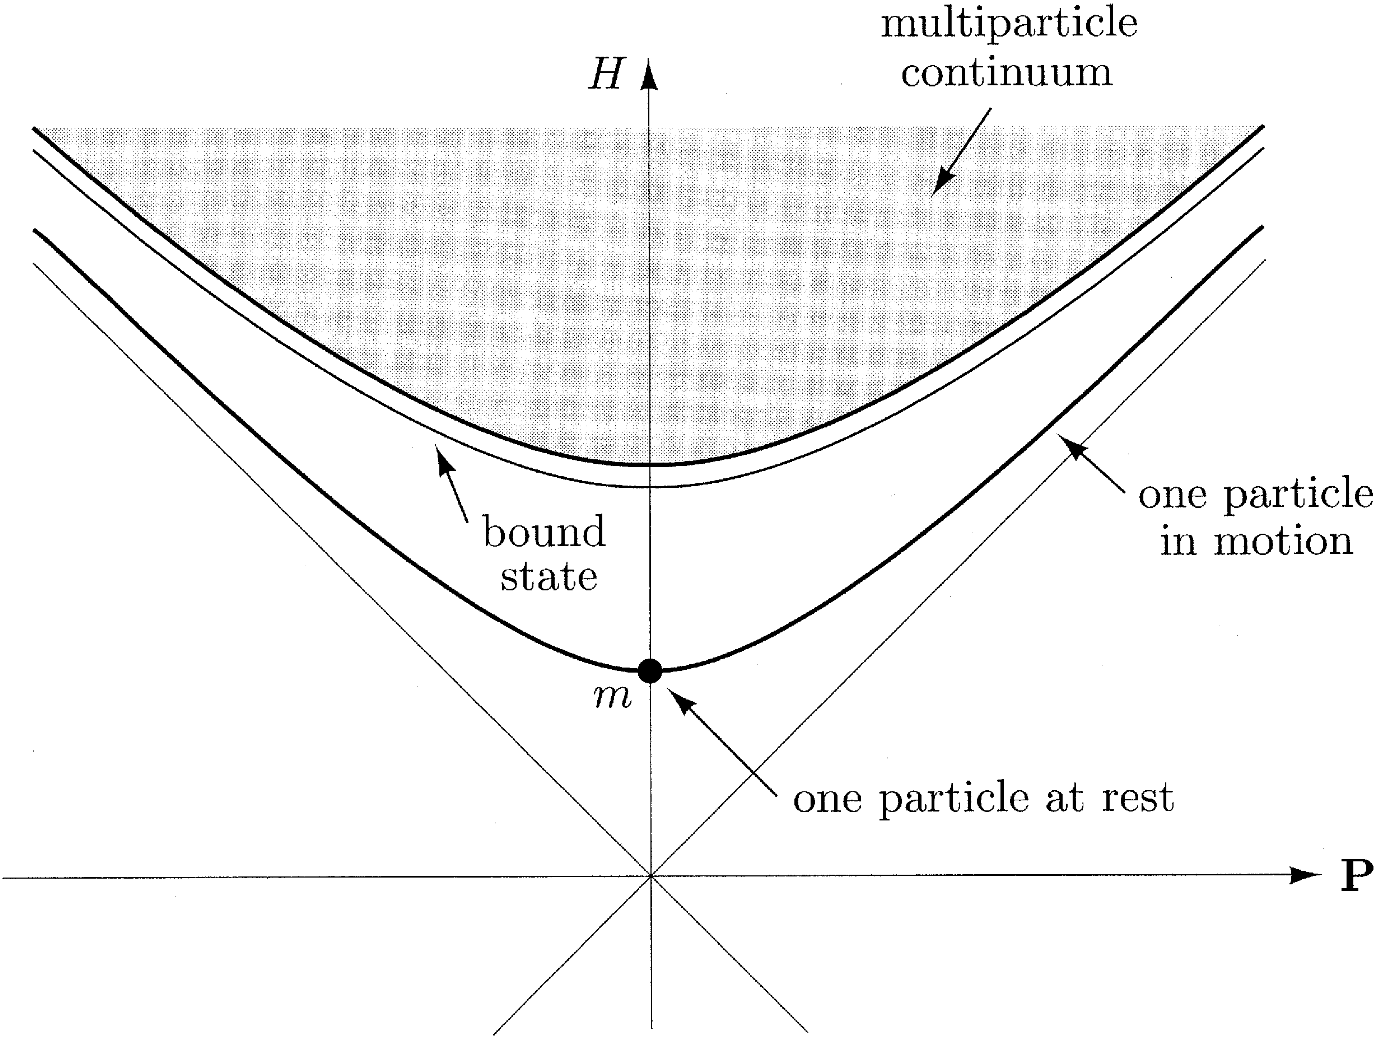
\includegraphics[width = 0.70 \textwidth]{images/mas-hyp.png}
  \caption{Hyperboloids in energy-momentum space formed by the eigenvalues of $ P^\mu = (H, \ve{P}) $.}
  \label{fig:mass-1}
\end{figure}

\begin{figure}[!ht]
  \centering
  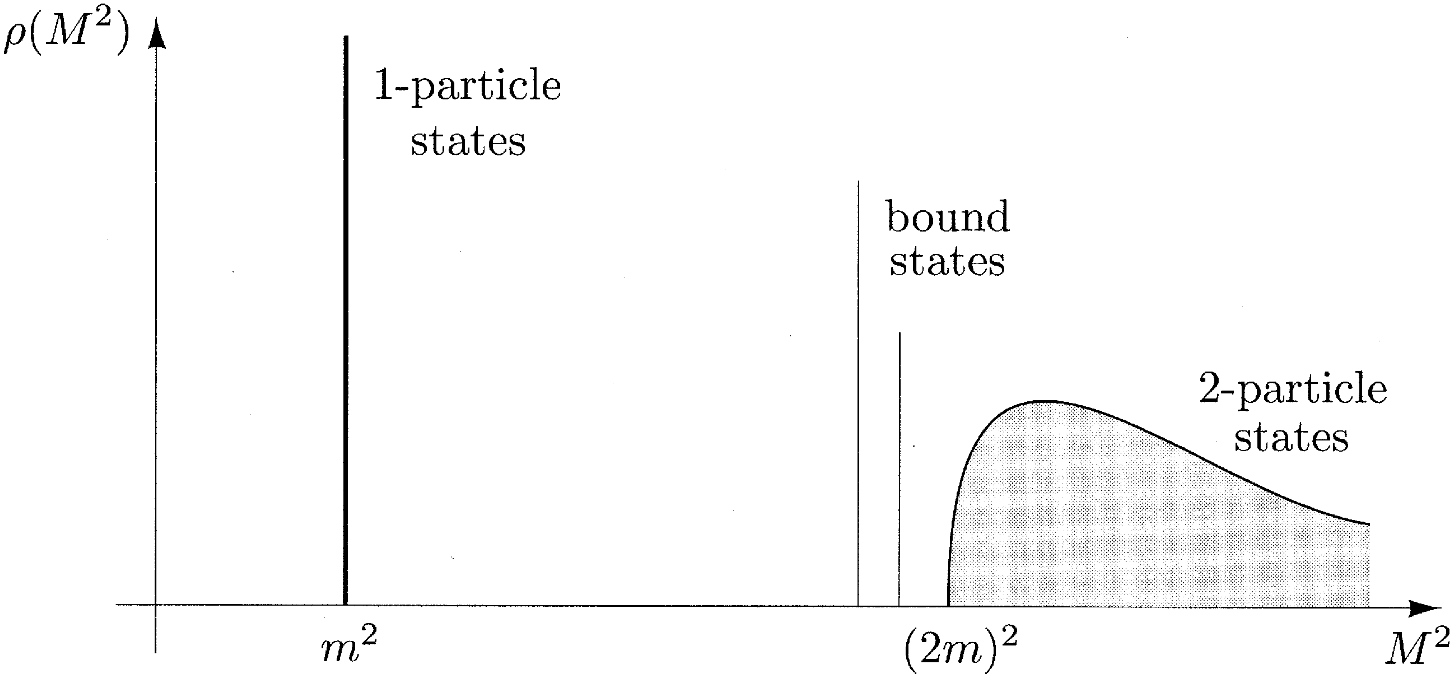
\includegraphics[width = 0.60 \textwidth]{images/spec-dens.png}
  \caption{Spectral density function for a typical interacting field theory.}
  \label{fig:mass-2}
\end{figure}

\begin{figure}[!ht]
  \centering
  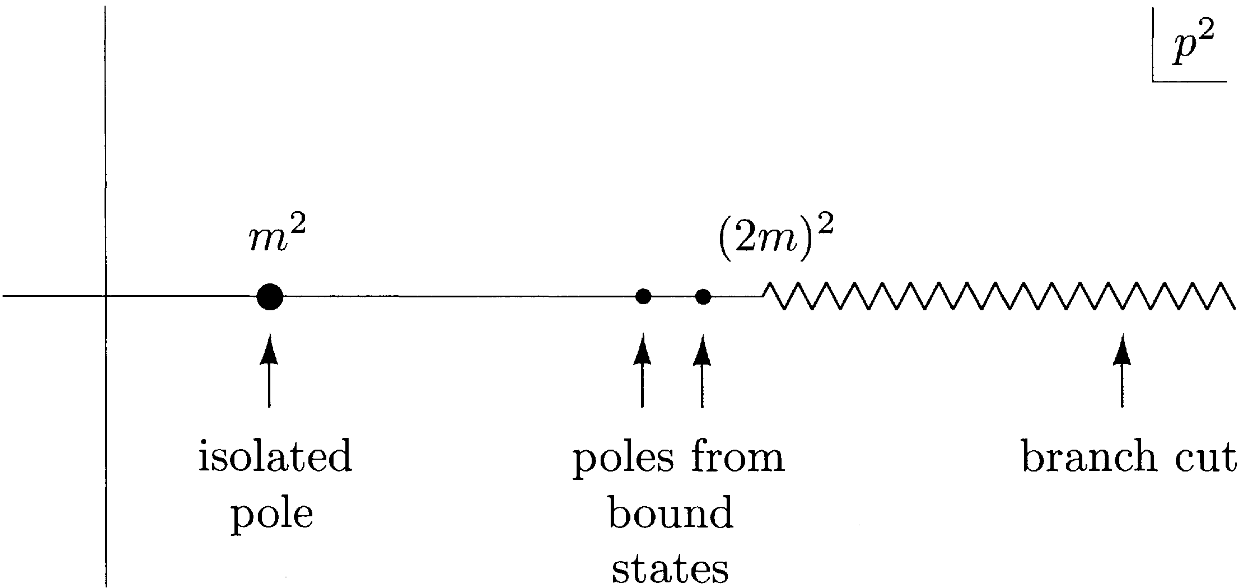
\includegraphics[width = 0.60 \textwidth]{images/poles.png}
  \caption{Analytic structure in the complex $ p^2 $-plane of $ \tilde{D}_\text{F}(p) $.}
  \label{fig:mass-3}
\end{figure}

As shown in Fig. \ref{fig:mass-2}, the one-particle states contribute to the spectral density with an isolated $ \delta $:
\begin{equation}
  \rho(M^2) = 2\pi \delta(M^2 - m^2) Z + (\text{terms with } M^2 \gtrsim (2m)^2)
\end{equation}
where $ Z $ is a number coming from the squared matrix element and it is called \bctxt{field-strength renormalization} (the same factor appearing in the LSZ reduction formula). Note that $ m $ is the physical mass of the particle, as opposed to the bare mass $ m_0 $ appearing in the Lagrangian. The Fourier transform of the $ 2 $-point Green function then is:
\begin{equation}
  \tilde{D}_\text{F}(p) = \frac{i Z}{p^2 - m^2 + i\epsilon} + \int_{\sim 4m^2}^\infty \frac{\dd M^2}{2\pi} \rho(M^2) \frac{i}{p^2 - M^2 + i\epsilon}
  \label{eq:corr-func-gen}
\end{equation}
The pole structure of $ \tilde{D}_\text{F}(p) $ is shown in Fig. \ref{fig:mass-3}: the first term gives an isolated simple pole in $ p^2 = m^2 $, while the second term contributes a branch cut beginning at $ p^2 = (2m)^2 $ (any two-particle bound states will appear as an additional $ \delta $ in $ \rho(M^2) $, i.e. additional an isolated pole below the branch cut). \eref{eq:corr-func-gen} is a direct generalization of \eref{eq:corr-func}: the former contains the field-strength renormalization $ Z = \abs{\braket{\lambda_0 | \phi(0) | 0}}^2 $, i.e. the probability for $ \phi(0) $ to create a given state from vacuum, while the latter has it implicitly, since in the free theory $ \abs{\braket{\ve{p} | \phi(0) | 0}}^2 = 1 $; moreover, \eref{eq:corr-func} is the amplitude of a single particle propagating from $ x $ to $ y $, as in the free theory $ \phi(0) $ can only create a single particle from vacuum, while \eref{eq:corr-func-gen} contains contributions from multiparticle intermediate states with a continuous mass spectrum.

\paragraph{Counterterms}

\eref{eq:corr-func-gen} has a single term which is singular at $ p^2 = m^2 $, and to eliminate the awkward residue $ Z $ it is possible to set:
\begin{equation}
  \phi \equiv \sqrt{Z} \phi_\text{r}
  \label{eq:phi-ren}
\end{equation}
This is the renormalized field (recall that it is equivalent to renormalize multiplicatively or additively).

\begin{proposition}{Renormalized $ \lambda \phi^4 $-theory}{}
  The renormalized Lagrangian of $ \lambda \phi^4 $-theory takes the form:
  \begin{equation}
    \lag = \frac{1}{2} \pa_\mu \phi_\text{r} \pa^\mu \phi_\text{r} - \frac{1}{2} m^2 \phi_\text{r}^2 - \frac{\lambda}{4!} \phi_\text{r}^4 + \frac{1}{2} \delta_Z \pa_\mu \phi_\text{r} \pa^\rho \phi_\text{r} - \frac{1}{2} \delta_m \phi_\text{r}^2 - \frac{\delta_\lambda}{4!} \phi_\text{r}^4
  \end{equation}
  with:
  \begin{equation}
    \delta_Z \equiv Z - 1
    \qquad \qquad
    \delta_m \equiv m_0^2 Z - m^2
    \qquad \qquad
    \delta_\lambda \equiv \lambda_0 Z^2 - \lambda
  \end{equation}
\end{proposition}

\begin{proofbox}
  \begin{proof}
    Inserting \eref{eq:phi-ren} into the Lagrangian of $ \lambda \phi^4 $-theory:
    \begin{equation*}
      \lag = \frac{1}{2} Z \pa_\mu \phi_\text{r} \pa^\mu \phi_\text{r} - \frac{1}{2} m_0^2 Z \phi_\text{r}^2 - \frac{\lambda_0}{4!} \phi_\text{r}^4
    \end{equation*}
    The isolation of counterterms is then trivial.
  \end{proof}
\end{proofbox}

This Lagrangian is composed of the standard $ \lambda \phi^4 $-theory Lagrangian, with renormalized field, mass and coupling constant, plus three counterterms: this is precisely the number of infinite constants appearing in diverging amplitudes of the theory. The Feynman rules for the renormalized theory are:
\begin{equation*}
  \begin{tikzpicture}[baseline=(r.base)]
    \begin{feynman}[inline=(r.base)]
      \vertex (a1) {};
      \vertex[right=4cm of a1] (a2) {};
      \vertex[below=4em of a1] (b1) {};
      \vertex[below=4em of a2] (b2) {};
      \vertex[below=2em of a1] (c1) {};
      \vertex[right=2cm of c1] (c2) {};

      \vertex[left = 2cm of c2] (d1) {};
      \vertex[right = 2cm of c2] (d2) {};

      \vertex[below=2.2em of a1] (r);

      \diagram* {
        (d1) -- [scalar, momentum = \(p\)] (d2),
      };
    \end{feynman}
  \end{tikzpicture}
  \quad = \quad \frac{i}{p^2 - m^2 + i\epsilon}
  \qquad
  \begin{tikzpicture}[baseline=(r.base)]
    \begin{feynman}[inline=(r.base)]
      \vertex (a1) {};
      \vertex[right=4cm of a1] (a2) {};
      \vertex[below=4em of a1] (b1) {};
      \vertex[below=4em of a2] (b2) {};
      \vertex[below=2em of a1] (c1) {};
      \vertex[right=2cm of c1, crossed dot] (c2) {};

      \vertex[left = 2cm of c2] (d1) {};
      \vertex[right = 2cm of c2] (d2) {};

      \vertex[below=2.2em of a1] (r);

      \diagram* {
        (d1) -- [scalar, momentum = \(p\)] (c2) -- [scalar] (d2),
      };
    \end{feynman}
  \end{tikzpicture}
  \quad = \quad i (p^2 \delta_Z - \delta_m)
\end{equation*}
\begin{equation*}
  \begin{tikzpicture}[baseline=(r.base)]
    \begin{feynman}[inline=(r.base)]
      \vertex (a1) {};
      \vertex[right=4cm of a1] (a2) {};
      \vertex[below=4em of a1] (b1) {};
      \vertex[below=4em of a2] (b2) {};
      \vertex[below=2em of a1] (c1) {};
      \vertex[right=2cm of c1, dot] (c2) {};

      \vertex[below=2.2em of a1] (r);

      \diagram* {
        (a1) -- [scalar] (c2),
        (b1) -- [scalar] (c2),
        (c2) -- [scalar] (a2),
        (c2) -- [scalar] (b2),
      };
    \end{feynman}
  \end{tikzpicture}
  \quad = \quad -i \lambda
  \qquad \qquad
  \begin{tikzpicture}[baseline=(r.base)]
    \begin{feynman}[inline=(r.base)]
      \vertex (a1) {};
      \vertex[right=4cm of a1] (a2) {};
      \vertex[below=4em of a1] (b1) {};
      \vertex[below=4em of a2] (b2) {};
      \vertex[below=2em of a1] (c1) {};
      \vertex[right=2cm of c1, crossed dot] (c2) {};

      \vertex[below=2.2em of a1] (r);

      \diagram* {
        (a1) -- [scalar] (c2),
        (b1) -- [scalar] (c2),
        (c2) -- [scalar] (a2),
        (c2) -- [scalar] (b2),
      };
    \end{feynman}
  \end{tikzpicture}
  \quad = \quad -i \delta_\lambda
\end{equation*}
To make the definition of the counterterms effective, the physical conditions which fix $ Z $, $ m $ and $ \lambda $ must be set, in order to set their value via comparison with experiments. The three \bctxt{renormalization conditions} are:
\begin{equation*}
  \begin{tikzpicture}[baseline=(r.base)]
    \begin{feynman}[inline=(r.base)]
      \vertex (a1) {};
      \vertex[right=4cm of a1] (a2) {};
      \vertex[below=4em of a1] (b1) {};
      \vertex[below=4em of a2] (b2) {};
      \vertex[below=2em of a1] (c1) {};
      \vertex[right=2cm of c1, blob] (c2) {};

      \vertex[left = 2cm of c2] (d1) {};
      \vertex[right = 2cm of c2] (d2) {};

      \vertex[below=2.2em of a1] (r);

      \diagram* {
        (d1) -- [scalar, momentum = \(p\)] (c2) -- [scalar] (d2),
      };
    \end{feynman}
  \end{tikzpicture}
  \quad = \quad \frac{i}{p^2 - m^2} + (\text{terms regular at } p^2 = m^2)
\end{equation*}
\begin{equation*}
  \begin{tikzpicture}[baseline=(r.base)]
    \begin{feynman}[inline=(r.base)]
      \vertex (a1) {};
      \vertex[right=4cm of a1] (a2) {};
      \vertex[below=4em of a1] (b1) {};
      \vertex[below=4em of a2] (b2) {};
      \vertex[below=2em of a1] (c1) {};
      \vertex[right=2cm of c1, blob] (c2) {};

      \vertex[below=2.2em of a1] (r);

      \diagram* {
        (a1) -- [scalar] (c2),
        (b1) -- [scalar] (c2),
        (c2) -- [scalar] (a2),
        (c2) -- [scalar] (b2),
      };
    \end{feynman}
  \end{tikzpicture}
  \quad = \quad -i \lambda
  \qquad \text{at} \qquad
  s = 4m^2 \,\,,\,\, t = u = 0
\end{equation*}
These physical conditions fix the pole and the residue of the $ 2 $-point Green function and the zero-momentum $ 2 \rightarrow 2 $ scattering amplitude: once loop integrals have been regularized, the $ \delta_Z $, $ \delta_m $ and $ \delta_\lambda $ are adjusted (renormalized) to satisfy the renormalization conditions and, after this adjustment, the amplitudes should be finite and independent of the regulator. This marks the successful renormalization of the theory\footnote{Note that in the $ \msb $ scheme the physical conditions are replaced by subtraction of poles: this means that the $ \msb $ mass $ m_{\msb} $ is not the pole of the $ 2 $-point Green function, hence it is not physically observable.}. \\
At $ \smo(\lambda) $ order only $ \delta_\lambda $ is non-trivial, as $ \delta_Z $ and $ \delta_m $ come into play only at $ \smo(\lambda)^2 $ with diagrams:
\begin{equation*}
  \begin{tikzpicture}[baseline = (r.base)]
    \begin{feynman}[inline = (r.base)]
      \vertex (x1) {};
      \vertex[below=3em of x1] (p1) {};
      \vertex[below=3em of p1] (x2) {};

      \vertex[right=3em of p1, dot] (v1) {};
      \vertex[right=5em of v1, dot] (v2) {};

      \vertex[right=3em of v2] (p2) {};
      \vertex[above=3em of p2] (x3) {};
      \vertex[below=3em of p2] (x4) {};

      \vertex[above=0.5em of v1] (r) {};

      \diagram* {
        (x1) -- [scalar] (v1),
        (x2) -- [scalar] (v1),
        (v2) -- [scalar] (x3),
        (v2) -- [scalar] (x4),

        (v1) -- [scalar, half left] (v2),
        (v2) -- [scalar, half left] (v1),
        (v1) -- [scalar] (v2),
      };
    \end{feynman}
  \end{tikzpicture}
  \quad + \quad
  \begin{tikzpicture}[baseline=(r.base)]
    \begin{feynman}[inline=(r.base)]
      \vertex (a1) {};
      \vertex[right=4cm of a1] (a2) {};
      \vertex[below=4em of a1] (b1) {};
      \vertex[below=4em of a2] (b2) {};
      \vertex[below=2em of a1] (c1) {};
      \vertex[right=2cm of c1, crossed dot] (c2) {};

      \vertex[left = 2cm of c2] (d1) {};
      \vertex[right = 2cm of c2] (d2) {};
      \vertex[above = 2cm of c2, empty dot] (d3) {};

      \vertex[above=1.1cm of c2] (r);

      \diagram* {
        (d1) -- [scalar] (c2) -- [scalar] (d2),
        (c2) -- [scalar, half left] (d3) -- [scalar, half left] (c2),
      };
    \end{feynman}
  \end{tikzpicture}
  \quad + \quad
  \begin{tikzpicture}[baseline=(r.base)]
    \begin{feynman}[inline=(r.base)]
      \vertex (a1) {};
      \vertex[right=4cm of a1] (a2) {};
      \vertex[below=4em of a1] (b1) {};
      \vertex[below=4em of a2] (b2) {};
      \vertex[below=2em of a1] (c1) {};
      \vertex[right=2cm of c1, crossed dot] (c2) {};

      \vertex[left = 2cm of c2] (d1) {};
      \vertex[right = 2cm of c2] (d2) {};

      \vertex[below=2.2em of a1] (r);

      \diagram* {
        (d1) -- [scalar] (c2) -- [scalar] (d2),
      };
    \end{feynman}
  \end{tikzpicture}
\end{equation*}
This means that:
\begin{equation}
  \delta_\lambda = 1 + \smo(\lambda)
  \qquad \qquad
  \delta_Z = 1 + \smo(\lambda^2)
  \qquad \qquad
  \delta_m = 1 + \smo(\lambda^2)
\end{equation}
agreeing with \secref{sssec:lag-count}. Tadpoles produces by the physical vertex (not the counterterm) should be considered too, but, as per \lref{lemma:tadpole-resumm}, they only contribute as a shift between $ m $ and $ m_0 $.










